\section{Results}\label{sec:results}

\subsection{Baselines: the price of admission}

Table~\ref{tab:baselines} and Figure~\ref{fig:baselines} report the
pre-registered baselines on the evaluation window. The ordering is
informative. The majority-class and constant policies (B1, B2) land
in the 44--56\% band---barely better than their own training-window
priors, a first sign that the evaluation window is not an easy era.
The reversal heuristic (B3) reaches 60.1\% but on the affirm/reverse
subset only, with an interval that warns against taking the point
estimate seriously. The per-justice ideology rules dominate: 55.8\%
at the case level (B4c) and \textbf{63.7\%} at the vote level (B4)
on the full evaluation window. On the transparent (sealed-excluded)
subset used for challenger comparison below, B4 scores 63.1\%
(n~$=$~1{,}522, CI [60.6; 65.5]).

\begin{table}[t]
\centering
\caption{Pre-registered baselines on the evaluation window
(OT2020--OT2023). Wilson 95\% intervals.}
\label{tab:baselines}
\small
\begin{tabular}{@{}lcc@{}}
\toprule
Baseline & Accuracy (\%) & 95\% CI \\
\midrule
B1---majority class (liberal) & 43.6 & [37.2; 50.1] \\
B2---always conservative & 56.4 & [49.9; 62.8] \\
B3---always reverse & 60.1 & [51.8; 67.9] \\
B4c---per-justice ideology, case level & 55.8 & [49.3; 62.2] \\
\textbf{B4---per-justice ideology, vote level} &
\textbf{63.7} & \textbf{[61.3; 65.9]} \\
\bottomrule
\end{tabular}
\end{table}

\begin{figure}[t]
\centering
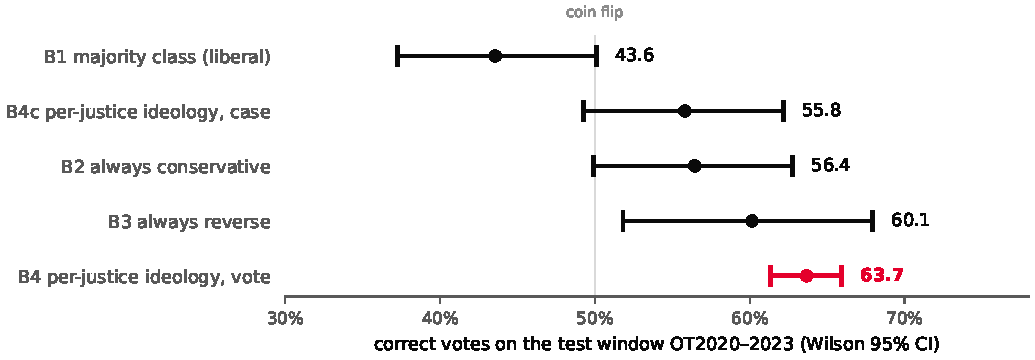
\includegraphics[width=\linewidth]{figures/fig2_baselines.pdf}
\caption{The number to beat. Wilson 95\% intervals for the five
baselines on the test window; B4 (red) is the vote-level bar of
63.7\%.}
\label{fig:baselines}
\end{figure}

\subsection{Pairwise agreement}

The descriptive baseline B5 measures how often two justices vote the
same way on their common cases. The extremes frame the scale:
Kavanaugh and Roberts agree on 94.6\% of their 333 common coded
votes (CI [91.6; 96.8]), while Sotomayor and Thomas agree on only
54.3\% of 518 (CI [50.0; 58.5])---statistically indistinguishable
from two justices flipping independent coins that share a slight
bias. Figure~\ref{fig:agreement} shows the full matrix, ordered by
mean agreement with the conservative anchor block (Thomas and
Alito). The block structure is visible without statistics: the
modern conservative five form a dark square in one corner, the
liberal three-plus in the other, and the two red-outlined extremes
are, on inspection, the two ends of the Court's ideological span.
This matrix is the empirical picture of what B4 compresses into one
bit per justice.

\begin{figure}[t]
\centering
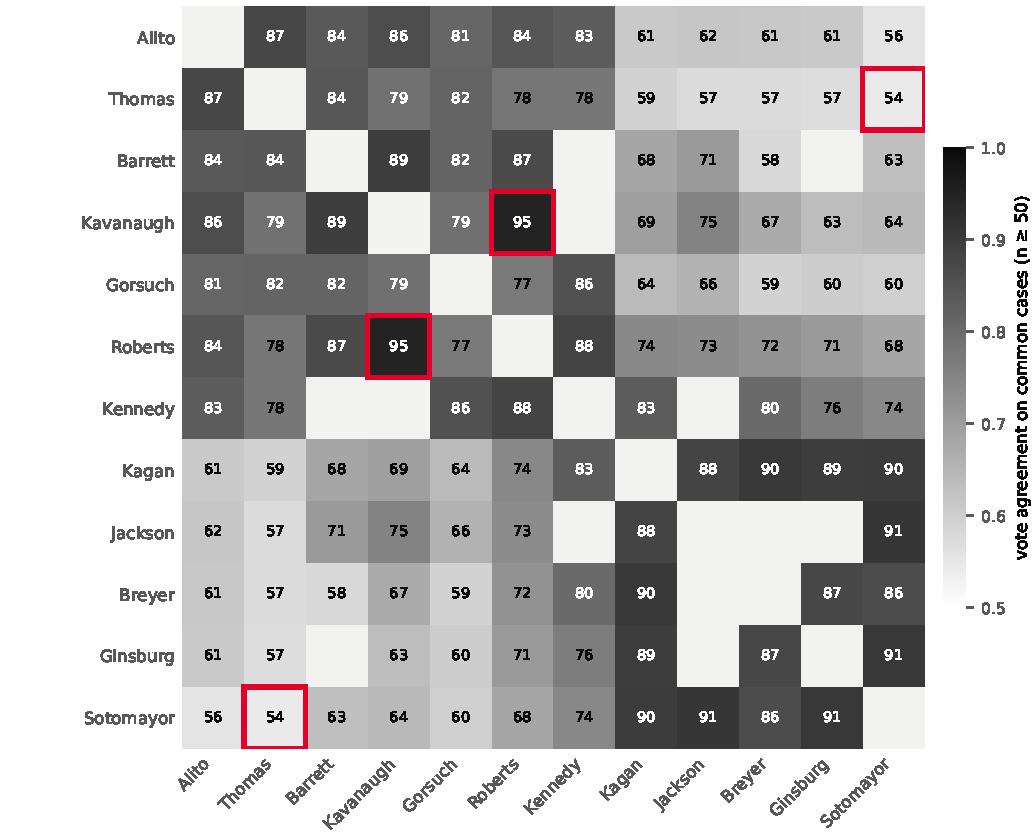
\includegraphics[width=0.92\linewidth]{figures/fig3_agreement.pdf}
\caption{Vote-level agreement across the 60 pairs with at least 50
common coded votes (values are percent agreement). Darker cells are
higher agreement; the diagonal is undefined. Red outlines mark the
closest (Kavanaugh--Roberts, 94.6\%) and widest (Sotomayor--Thomas,
54.3\%) pairs. Ordering is by mean agreement with the conservative
anchor block.}
\label{fig:agreement}
\end{figure}

\subsection{M3a: the structured challengers---and the bar holds}

The first trained condition, M3a, asks whether the structured,
pre-decision attributes of a case---issue area, lower-court
disposition, term, and oral-argument duration, joined with justice
identity---predict vote direction better than the one-bit
ideological rule. Three challengers were trained on the
sealed-excluded training window with grouped cross-validation for
all hyper-parameter choice: an additive logistic regression (M3a-LR),
the same with explicit justice$\times$issue interactions (M3a-IX),
and a histogram gradient-boosting classifier that learns
interactions natively (M3a-GB).

\begin{table}[t]
\centering
\caption{M3a challengers vs.\ the bar, transparent test
(sealed-excluded; $n=1{,}522$ rows common to all rows where B4 is
defined). McNemar exact test against B4's paired predictions.}
\label{tab:m3a}
\small
\begin{tabular}{@{}lcccc@{}}
\toprule
Model & CV (\%) & Test (\%) & 95\% CI & $p$ \\
\midrule
M3a-LR (additive) & 56.2 & 58.6 & [56.1; 61.1] & 0.002 \\
M3a-GB (boosting) & 56.1 & 59.8 & [57.3; 62.2] & 0.009 \\
M3a-IX (interactions) & 57.1 & 60.4 & [57.9; 62.8] & 0.047 \\
\textbf{B4 (bar)} &---& \textbf{63.1} & \textbf{[60.6; 65.5]} &
--- \\
\bottomrule
\end{tabular}
\end{table}

\begin{figure}[t]
\centering
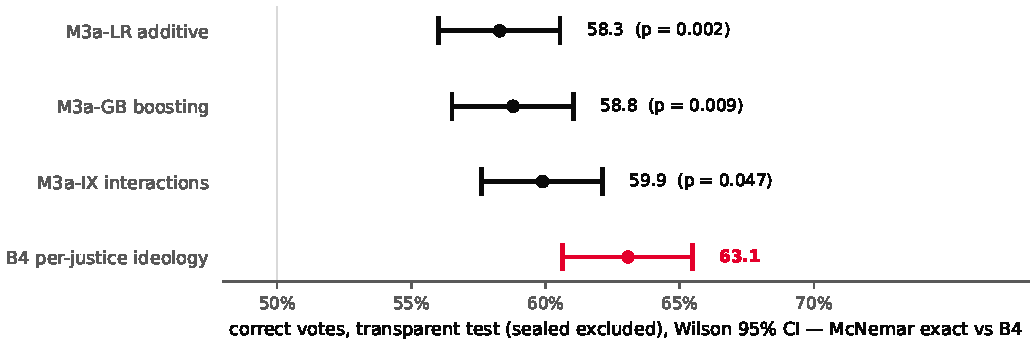
\includegraphics[width=\linewidth]{figures/fig4_m3a.pdf}
\caption{The first challenger fails against the bar. Wilson 95\%
intervals on the common rows; $p$-values are exact McNemar tests
against B4's paired predictions.}
\label{fig:m3a}
\end{figure}

Table~\ref{tab:m3a} and Figure~\ref{fig:m3a} give the result: every
challenger lands between 58.6\% and 60.4\% on the common rows, and
every comparison against B4 favors the bar (McNemar exact
$p \le 0.047$). The failure is not an artifact of regularization
strength or model family; it is robust across three families and
survives the interaction model that the site's per-justice
domain-divergence displays would suggest. It is also not a power
issue in the usual direction---the challengers are significantly
\emph{worse}, not merely insignificantly different.

The ablation in Table~\ref{tab:ablation} locates the failure
precisely. Removing justice identity from the feature set collapses
cross-validated accuracy from 56.2\% to 47.6\%---below the class
base rate---while removing any other feature group \emph{improves}
it (issue area is the most harmful to keep, at $+1.7$ points when
dropped). In other words, on this window, \emph{who} votes is
signal; \emph{what the case is about} is noise. The structured
challenger did not fail because the metadata was too thin; it
failed because the only stable generalizable structure in the data
is the attitudinal bit that B4 already uses.

\begin{table}[t]
\centering
\caption{Feature-group ablation (grouped 5-fold CV on the training
window, additive logistic regression).}
\label{tab:ablation}
\small
\begin{tabular}{@{}lc@{}}
\toprule
Feature set & CV accuracy (\%) \\
\midrule
Full (justice, issue, lc, term, duration) & 56.2 \\
drop justice identity & 47.6 \\
drop issue area & 57.9 \\
drop lower-court disposition & 56.7 \\
drop term & 56.5 \\
drop argument duration & 56.1 \\
\bottomrule
\end{tabular}
\end{table}

The case-level reading is the same. Simulating each case's outcome
as the majority of the challenger's predicted votes yields 58.3\%
(CI [51.5; 64.9]) on the transparent subset---above the case-level
ideological baseline (55.8\%), but the interval is wide enough that
the honest summary is ``not distinguishable'', and the vote-level
failure stands regardless.

\subsection{What the null prices}

Read together, the results give the experiment its current shape.
The predictable component of a justice's vote on this window is, to
the resolution that nine terms of structured data can detect, the
justice's ideological direction---exactly what the attitudinal
model predicts and exactly what B4 encodes. The additional
information that would be needed to beat 63.7\%, if it exists in
public data at all, is therefore not in the metadata: it must be in
the \emph{text}---the briefs, the transcript, the opinion language
itself. That is where the pre-registered conditions A--C operate,
and the M3a null result is what makes them the critical path rather
than a side quest: the structured ceiling is now empirically priced,
so any future claim of textual signal is a claim against a known,
pre-registered number.
